\section{SeeDB Frontend}
\label{subsec:seedb_frontend}

TThe \SeeDB\ frontend, designed as a thin client, performs two main functions: it
allows the analyst to issue a query to \SeeDB, 
and it visualizes the results (views) produced by the \SeeDB\
backend.
To provide the analyst maximum flexibility in issuing queries, \SeeDB\
provides the analyst with three
mechanisms for specifying an input query: 
(a) directly filling in SQL into a text box, 
(b) using a query builder tool that allows analysts
unfamiliar with SQL to formulate queries through a form-based interface, and (c)
using pre-defined query templates which encode commonly performed operations,
e.g., selecting outliers in a particular column. 
%We find that pre-defined query
%templates are particularly useful since analysts are often interested in
%anomalous data points.

Once the analyst issues a query via the \SeeDB\ frontend, the backend
evaluates various views and delivers the most interesting ones (based on
utility) to the frontend.
For each view delivered by the backend, the frontend creates a visualization
based on parameters such as the data
type (e.g. ordinal, numeric), number of distinct values, and semantics (e.g.
geography vs. time series).
The resulting set of visualizations is displayed to the analyst who can then
easily examine these ``most interesting'' views at a glance, explore specific views in
detail via drill-downs, 
%by hovering and clicking on various portions of the view, 
and study metadata for each view (e.g. size of result, sample data, value with
maximum change and other statistics). 
%The analyst can also slice-and-dice views further by performing drill-downs on
%specific attributes in the view. 
Figure~\ref{fig:frontend1} shows a screenshot of the \SeeDB\ frontend (showing
the query builder) in action.
 
\begin{figure}[htb]
\vspace{-10pt}
\centerline{
\hbox{\resizebox{5cm}{!}{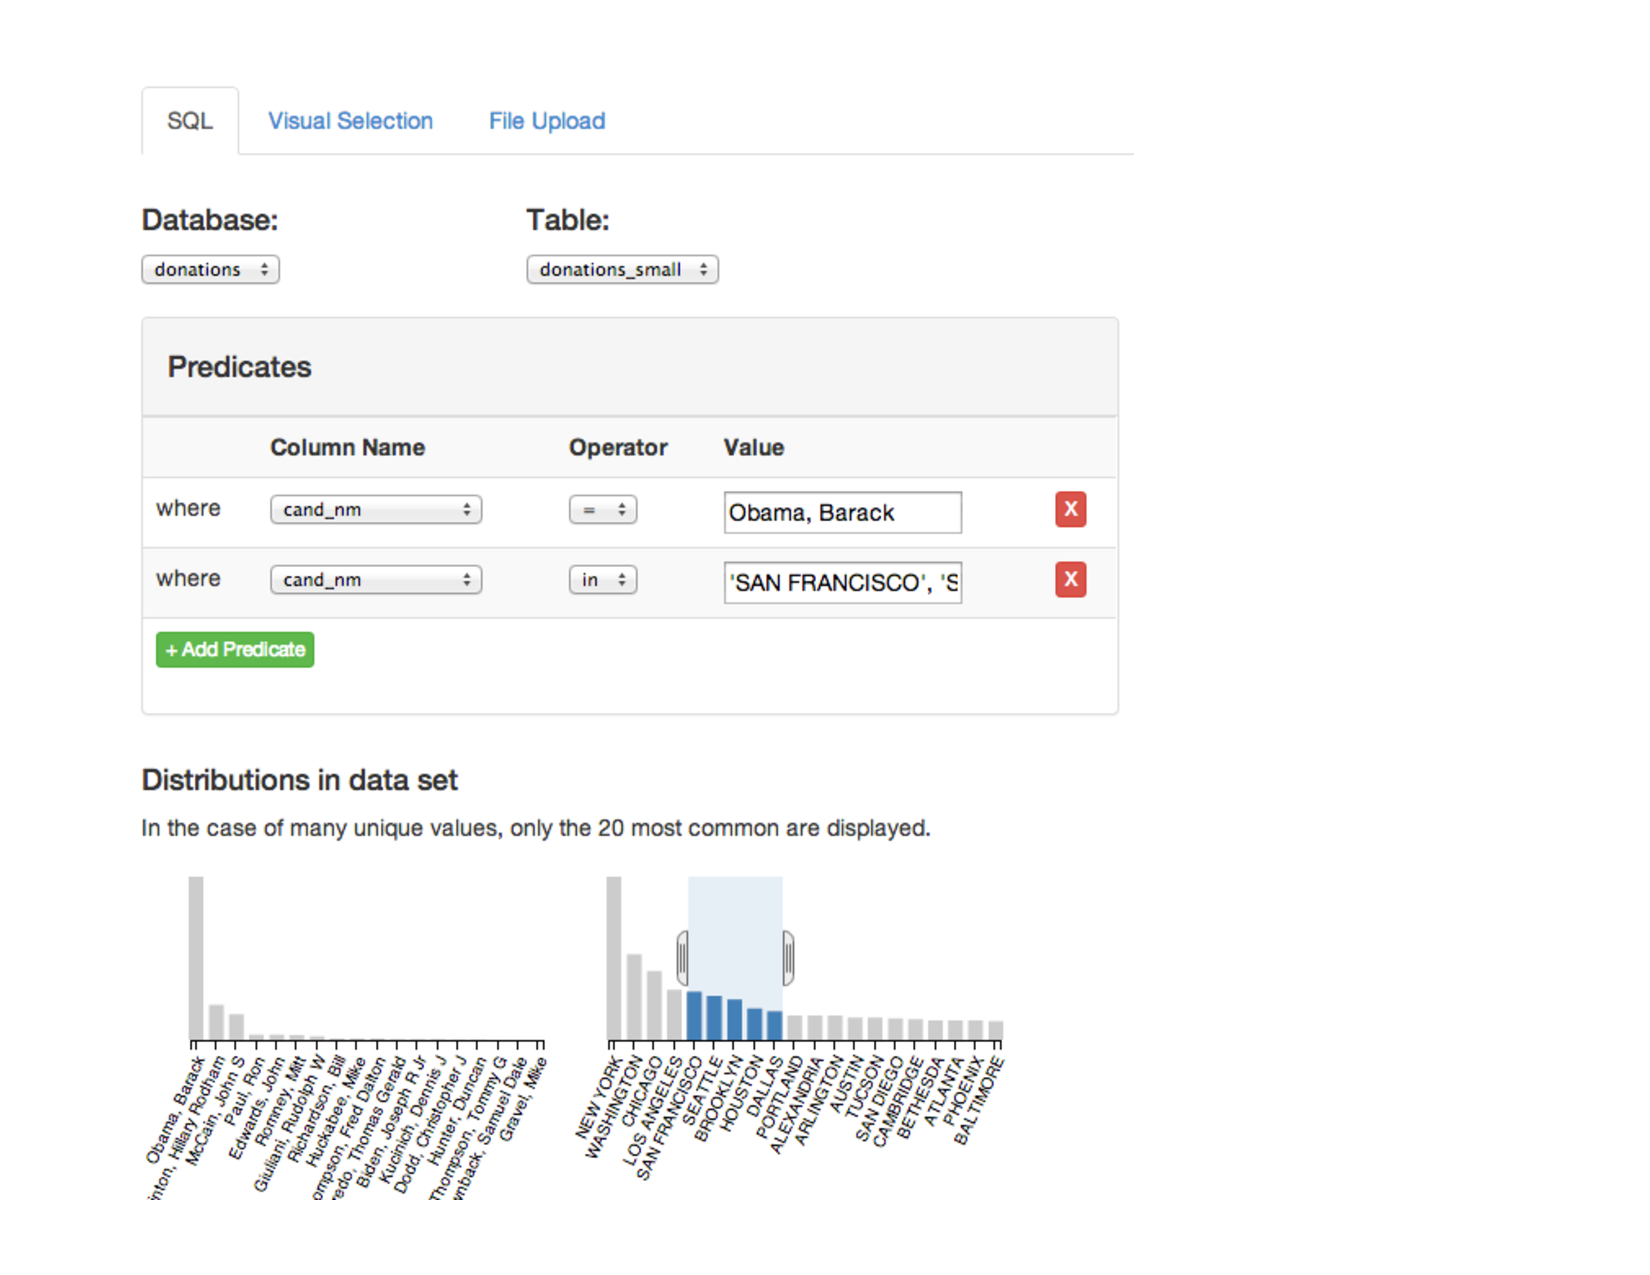
\includegraphics[trim=15mm 0mm 120mm 0mm,
clip=true]{Images/sql_builder.pdf}}}
\hbox{\resizebox{!}{6cm}{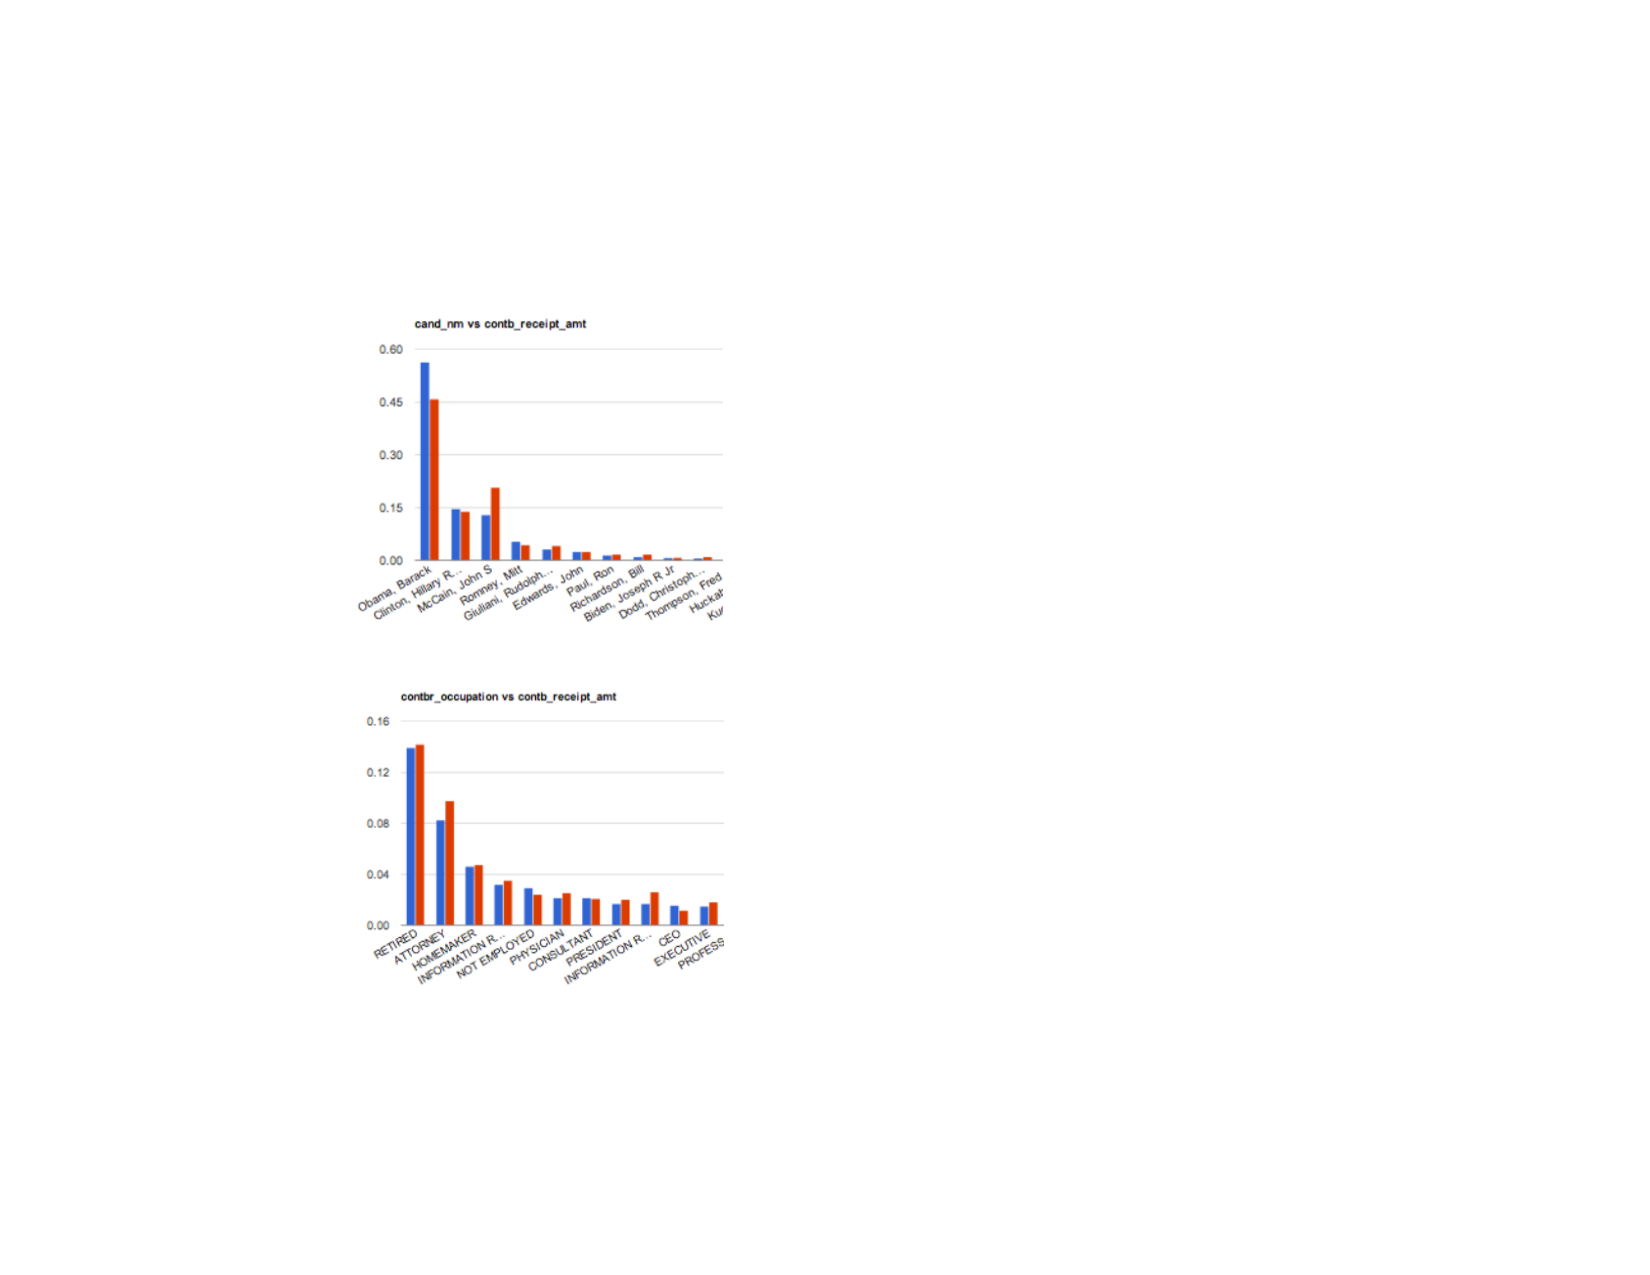
\includegraphics[trim=50mm 30mm 150mm 52mm,
clip=true]{Images/viz_panel.pdf}}}}
\caption{SeeDB Frontend: Query Builder (left) and Example Visualizations
(right)}
\label{fig:frontend1}
\vspace{-10pt}
\end{figure} 

\mpv{Interactivity. Ship all data to client?}